\newpage
%**************************************************************
\chapter{Casi d'uso}
\label{cap:Casi d'uso}

	\begin{figure}[ht]
		\centering
		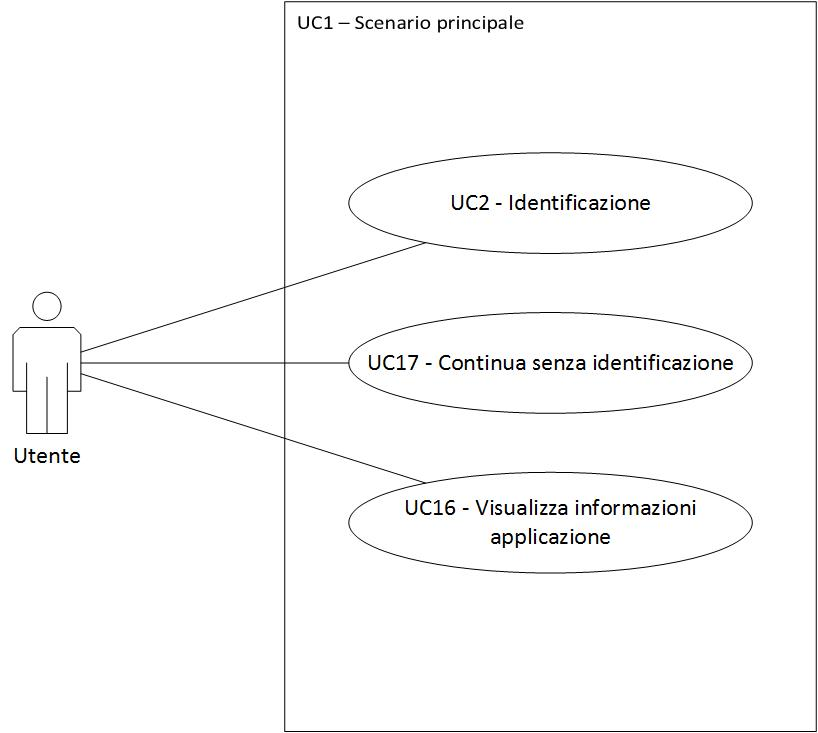
\includegraphics[scale=0.35]{immagini/analisi/UC01_scenario_principale.jpg}
		\caption{\textit{Caso d'uso UC01 - Scenario principale}}
	\end{figure}\FloatBarrier
	
	\begin{center}
		\begin{tabularx}{\textwidth}{p{3cm} p{9.30cm}}
			\hline
			\textbf{UC01} & \textbf{Scenario principale} \\
			\hline
			\textit{Attore principale} & Utente \\
			\hline
			\textit{Precondizioni} & L’applicazione è stata avviata\\
			\hline
			\textit{Postcondizioni} & L’utente ha selezionato una azione disponibile\\
			\hline
			\textit{Scenario principale} & L’utente decide se utilizzare l’applicazione senza avere un profilo creato, oppure decide di identificarsi con le proprie credenziali fornite dall’azienda. E’ possibile anche che l’utente scelga di visualizzare le informazioni riguardanti l’applicazione, oppure un tutorial su come funziona l’applicazione (opzionale).\\
			\hline
		\end{tabularx}
	\end{center}
	
	\begin{figure}[ht]
		\centering
		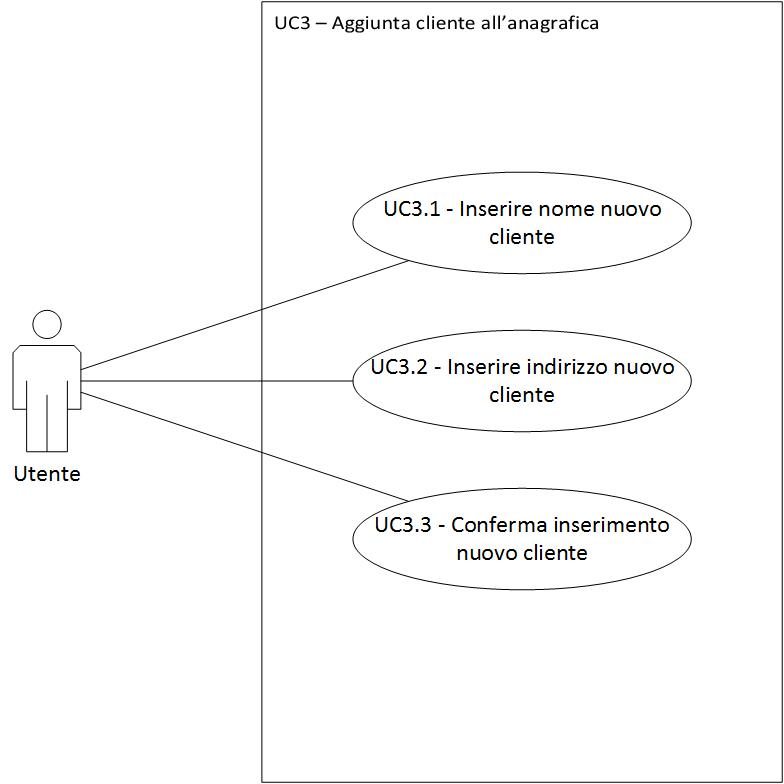
\includegraphics[scale=0.35]{immagini/analisi/UC03_aggiunta_cliente_anagrafica.jpg}
		\caption{\textit{Caso d'uso UC03 - Aggiunta anagrafica cliente}}
	\end{figure}\FloatBarrier
	
		\begin{center}
			\begin{tabularx}{\textwidth}{p{3cm} p{9.30cm}}
				\hline
				\textbf{UC03} & \textbf{Aggiunta anagrafica cliente} \\
				\hline
				\textit{Attore principale} & Utente \\
				\hline
				\textit{Precondizioni} & L’utente non ha un’identificazione e ha scelto di inserire un nuovo cliente\\
				\hline
				\textit{Postcondizioni} & \L’utente ha aggiunto un cliente nella sua anagrafica\\
				\hline
				\textit{Scenario principale} & L’utente inserisce un nuovo cliente nella sua anagrafica\\
				\hline
				\textit{Estensioni} & L’utente non inserisce tutti i dati necessari, quindi il sistema non gli permette di confermare l’inserimento del nuovo cliente, inoltre gli visualizza il motivo dell’errore in modo specifico. Dall’errore l’utente può decidere se continuare o concludere senza inserire l’utente.\\
				\hline
			\end{tabularx}
		\end{center}
	
	\begin{figure}[ht]
		\centering
		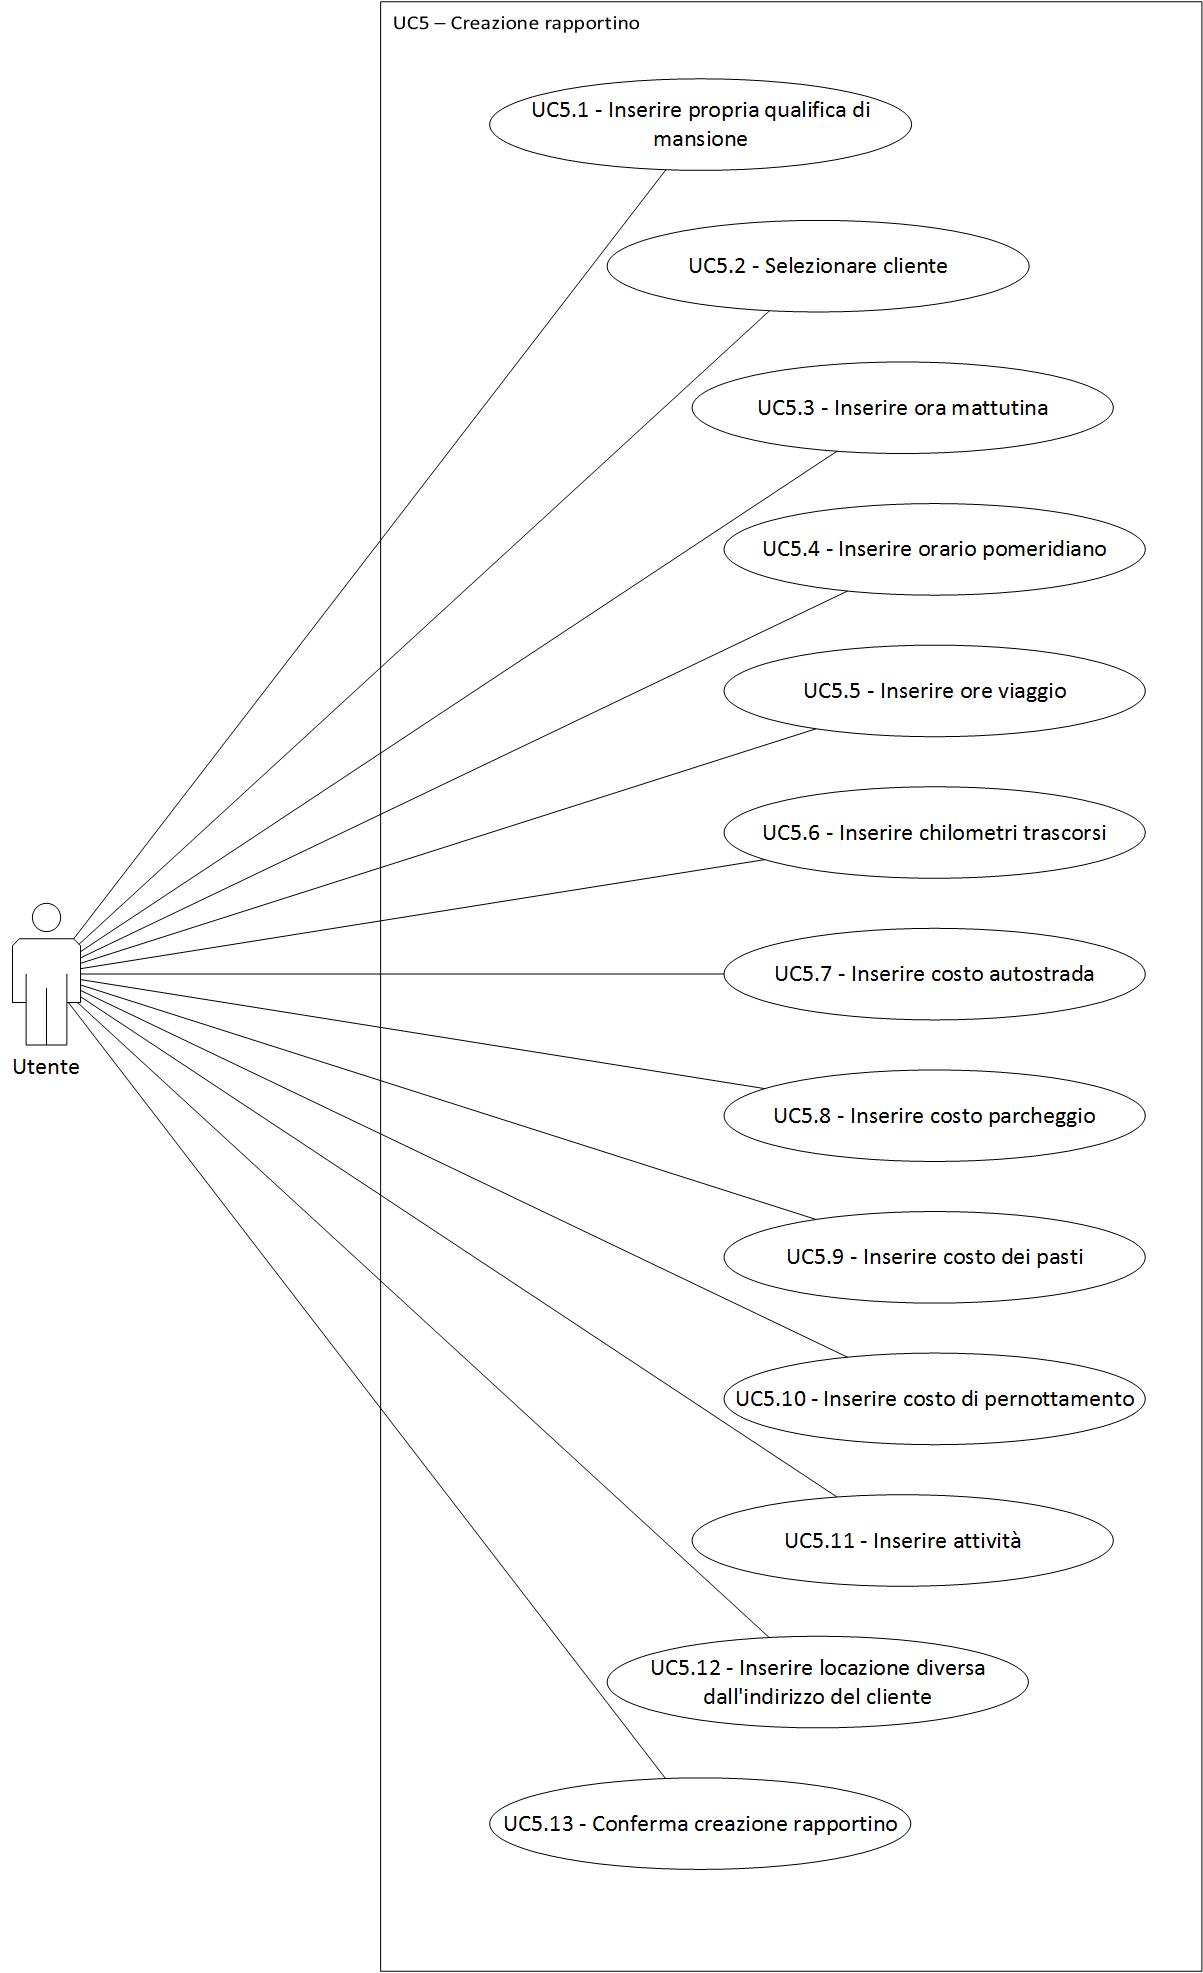
\includegraphics[scale=0.35]{immagini/analisi/UC05_creazione_rapportino_utente.jpg}
		\caption{\textit{Caso d'uso UC05 - Inserimento dati per creazione rapportino - Utente}}
	\end{figure}\FloatBarrier
	
		\begin{center}
			\begin{tabularx}{\textwidth}{p{3cm} p{9.30cm}}
				\hline
				\textbf{UC05} & \textbf{Inserimento dati per creazione rapportino} \\
				\hline
				\textit{Attore principale} & Utente \\
				\hline
				\textit{Precondizioni} & L’utente ha selezionato la creazione di un nuovo rapportino, il sistema mostra a video la form per l’inserimento dei dati\\
				\hline
				\textit{Postcondizioni} & L’utente ha creato un rapportino\\
				\hline
				\textit{Scenario principale} & L’utente inserisce tutti i dati necessari per la creazione di un nuovo rapportino, lo conferma e il sistema mostra un messaggio di buon fine. Nel messaggio verrò chiesto se l’utente vuole inviare il rapportino appena creato.\\
				\hline
				\textit{Estensioni} & L’utente non inserisce tutti i campi obbligatori impedendo al sistema di creare un rapportino, quindi il sistema avvisa con un messaggio di errore specifico. Nel messaggio d’errore verrà fornito all’utente la possibilità di continuare oppure di concludere senza la creazione del rapportino.\\
				\hline
			\end{tabularx}
		\end{center}
	
	\begin{figure}[ht]
		\centering
		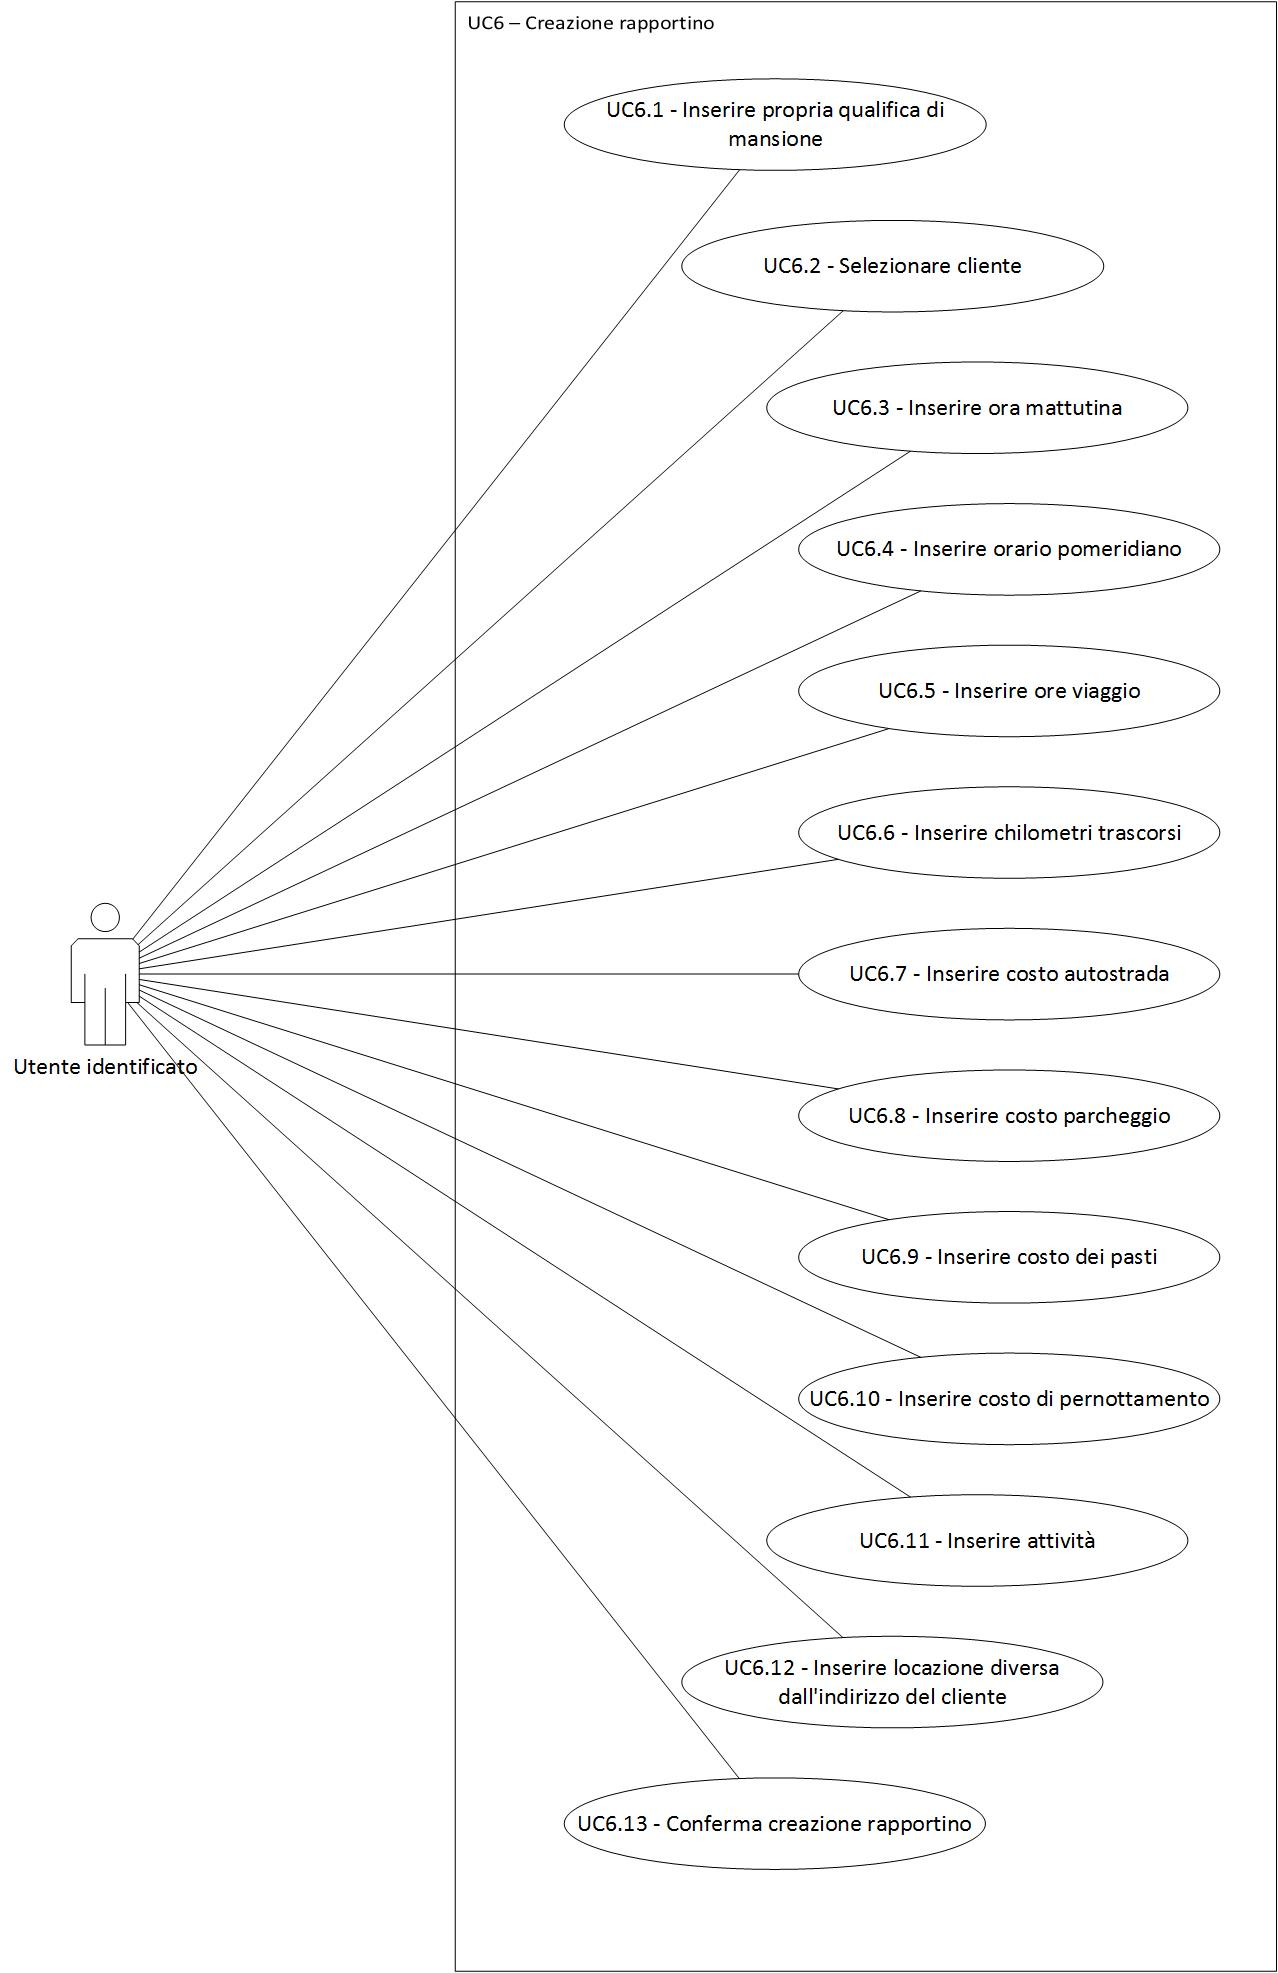
\includegraphics[scale=0.35]{immagini/analisi/UC06_creazione_rapportino_identificato.jpg}
		\caption{\textit{Caso d'uso UC06 - Inserimento dati per creazione rapportino - Utente identificato}}
	\end{figure}\FloatBarrier
	
		\begin{center}
			\begin{tabularx}{\textwidth}{p{3cm} p{9.30cm}}
				\hline
				\textbf{UC06} & \textbf{Creazione rapportino} \\
				\hline
				\textit{Attore principale} & Utente identificato\\
				\hline
				\textit{Precondizioni} & L’utente identificato ha selezionato la creazione di un nuovo rapportino, il sistema mostra a video la form per l’inserimento dei dati\\
				\hline
				\textit{Postcondizioni} & L’utente ha creato un rapportino\\
				\hline
				\textit{Scenario principale} & L’utente inserisce tutti i dati necessari per la creazione di un nuovo rapportino, lo conferma e il sistema mostra un messaggio di buon fine. Nel messaggio verrò chiesto se l’utente vuole inviare il rapportino appena creato.\\
				\hline
				\textit{Estensioni} & L’utente non inserisce tutti i campi obbligatori impedendo al sistema di creare un rapportino, quindi il sistema avvisa con un messaggio di errore specifico. Per essere creato, un rapportino necessita almeno l’inserimento di un cliente e della mansione.\\
				\hline
			\end{tabularx}
		\end{center}